\documentclass[12pt]{report}

\usepackage[T1]{fontenc}
\usepackage[utf8]{inputenc}
\usepackage{graphicx}

\begin{document}
 
\begin{center}
{\Huge Diagrama electrico de la interfaz de potencia}
\end{center}
\begin{center}

\includegraphics[scale=1]{../../../../Downloads/upzmg.jpg} 
\end{center} 
{\Huge Enesto Alonso Partida López\\Agustin Ascencio de Leon\\Maria de Lourdes Gomez Islas\\ \\Universidad Politecnica De La Zona Metropolitana De Guadalajara\\ Mecatronica 4 A\\ Septiembre-diciembre 2019}
\date{  de noviembre  2019}
 
\newpage

{\huge \textbf{INTRODUCCION:}\\}\\


{\large Realizar un aumento, disminución o ambos en el voltaje de salida con respecto a la entrada esto mediante los circuitos conocidos como convertidores de CD-CD (Boost, Buck y Buck/Boost) los cuales permitirán realizar esta tarea para aumentar o disminuir el voltaje de salida .}\\
 

{\huge \textbf{OBJETIVO}\\}\\


{\large Lograr el aumento del voltaje de entrada de 1.5V a 3.3V y la disminución de los voltajes 5V y 12V a un voltaje de salida de 3.3V.}\\



{\huge \textbf{MARCO TEORICO}\\}\\


{\large Un convertidor reductor (convertidor reductor) es un convertidor de potencia CC a CC que reduce el voltaje (mientras aumenta la corriente) desde su entrada (suministro) hasta su salida (carga). Es una clase de fuente de alimentación de modo conmutado (SMPS) que normalmente contiene al menos dos semiconductores (un diodo y un transistor, aunque los convertidores buck modernos con frecuencia reemplazan el diodo con un segundo transistor utilizado para la rectificación síncrona) y al menos un elemento de almacenamiento de energía , un condensador, inductor o los dos en combinación. Para reducir la fluctuación de voltaje, los filtros hechos de condensadores (a veces en combinación con inductores) normalmente se agregan a la salida y el filtro (filtro del lado de la carga) de dicho convertidor.}
\begin{center}
\begin{figure}[hbtp]
\caption{Convertidor Buck}
\centering
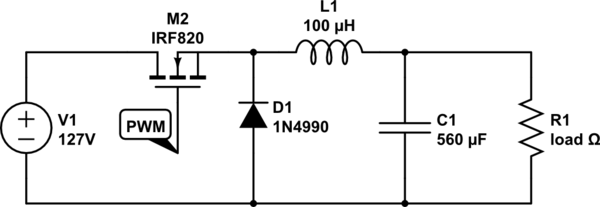
\includegraphics[scale=1]{../../../../Downloads/descragas/buck.png}
\end{figure}

\end{center}

\newpage
{\large Un convertidor elevador (convertidor elevador) es un convertidor de potencia CC a CC que aumenta el voltaje (mientras reduce la corriente) desde su entrada (suministro) hasta su salida (carga). Es una clase de fuente de alimentación de modo conmutado (SMPS) que contiene al menos dos semiconductores (un diodo y un transistor) y al menos un elemento de almacenamiento de energía: un condensador, inductor o los dos en combinación. Para reducir la fluctuación de voltaje, los filtros hechos de condensadores (a veces en combinación con inductores) normalmente se agregan a la salida y el filtro (filtro del lado de la carga) de dicho convertidor.}
\begin{center}
\begin{figure}[hbtp]
\centering
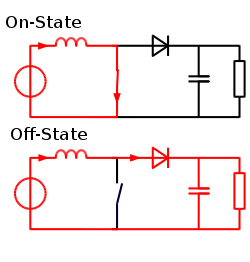
\includegraphics[scale=0.5]{../../../../Downloads/descragas/boost.png}
\caption{Convertidor Bock}
\end{figure}

\end{center}
\newpage
{\large El convertidor buck-boost es un tipo de convertidor de CC a CC que tiene una magnitud de voltaje de salida que es mayor o menor que la magnitud del voltaje de entrada. Es equivalente a un convertidor de retorno que utiliza un solo inductor en lugar de un transformador.}
\begin{center}
\begin{figure}[hbtp]
\centering
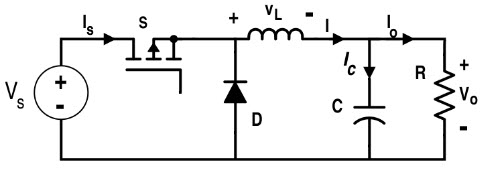
\includegraphics[scale=1]{../../../../Downloads/descragas/buck7bost.jpg}
\caption{Convertidor Buck/Boost}
\end{figure}

\end{center}
\newpage

{\huge \textbf{MATERIALES}\\}\\


\begin{enumerate}
\item Protoboard
\item Bobina
\item Resistencias
\item Placa Arduino
\item Diodo 1N4001
\item Fuente de Voltaje
\item Clabe Para Protoboard
\item Caimanes
\item Capacitores
\item Transistores o MOSFET 
\end{enumerate}


{\huge \textbf{Desarrollo}\\}\\
{\large \begin{enumerate}
\item Se comenzará con el armado de la bobina, esto en el caso de que no se tenga, a un clavo de hierro será necesario enrollar alambre de cobre alrededor de dicho clavo, para lograr hacer una bobina.
\item Una vez que se tiene la bobina, junto con todos sus materiales se procederá a armar tres circuitos los cuales serán el convertidor Buck, Boost y Buck/Boost, los cuales permitirán cambiar el voltaje de salida.
\item Se comenzará con el armado del convertidor Buck el cual necesita un MOSFET, una bobina y un par de capacitores junto con resistencias y un diodo.
\item posterior mente será necesario realizar el Boost, el cual necesita una bobina, un MOSFET, capacitor, resistencia y diodos.
\item por último será necesario realizar el convertidor Buck/Boost el cual constará de dos MOSFET, un embobinado, dos diodos y un par de capacitores junto con resistencias.
\item una vez realizados los circuitos, será necesario probarlos que funcionen correctamente.

\end{enumerate}}

{\huge \textbf{Resultados obtenidos}\\}\\
{\large El primer Circuito que es el Buck logro reducir el voltaje de entrada el cual fue de 5V a un volteje de salida de 3.43V, esto con un aumento y una disminución de décimas, el Boost solo logro mantener el voltaje de entrada mas no se logró superar quizás por que le falto colocar el potenciómetro que elevaría el voltaje de entrada el cual fue de 1.5 y solo logramos una salida de 1.4V y por último el Buck/Boost logro reducir el voltaje de entrada que eran 12V a una voltaje de salida de casi 3.45V, por lo cual se logró el objetivo planteado en la práctica.  }\\


{\huge \textbf{Conclusión}\\}\\
{\large Este tipo de circuitos convertidores serán muy útiles en el proyecto final del año, ya que en alguna ocasión se necesitará realizar una disminución del voltaje o bien un aumento para lograr mover los motores del dron, así como se tiene una noción de cómo hacer que el voltaje disminuya o aumente para ingresarlo a un circuito as adelante en el cual solo se cuente con un voltaje fijo y se necesite otro muy distinto.}
\newpage
{\huge \textbf{Bibliografia:}\\}\\

@online{Electronoobs,
author = {Anonimo},
title = {Convertidores DC-DC},
year = {2016},
URL = {https://www.electronoobs.com},
OPTlanguage = {español},

}

\end{document}